% !TEX encoding = UTF-8
% !TEX TS-program = pdflatex
% !TEX root = ../tesi.tex

%**************************************************************
\chapter{Strumenti utilizzati}
\label{cap:strumenti-utilizzati}
%**************************************************************

\section{Strumenti di sviluppo}
\subsection{Visual Studio Code}
\begin{figure}[ht]
    \centering
    
\includegraphics[height=2cm]{vsc_logo}
    \caption{Logo di Visual Studio Code}
\end{figure} \aCapo{}
\vsc{} è un editor per codice sorgente, sviluppato da \textit{Microsoft} servendosi del framework \textit{Electron}, disponibile per Windows, Linux e macOS. Le sue funzionalità comprendo supporto per debugging, syntax highlighting, intelligent code completion, snippets, code refactoring, e integrazione con Git. \\
Gli utenti possono configurare tema, macro, preferenze e installare estensioni che ne aumentano le funzionalità aggiungendo ad esempio il supporto ai maggiori linguaggi di porgrammazione attualmente presenti.\\
Nella \textit{Stack Overflow 2021 Developer Survey}, \vsc{} è risultato essere l'IDE più popolare, adottato dal 70\% degli intervistati. {\tiny Fonte: \href{https://en.wikipedia.org/wiki/Visual_Studio_Code}{Wikipedia}}\\
\E{} inoltre presente e molto comoda l'estensione di \flutter{} che, tra le altre cose, permette di gestire direttamente in gui i vari dispositivi (smartphone, browser o emulatore) sui quali installare e lanciare l'app che si sta programmando.

\subsection{Android Studio}
\begin{figure}[ht]
    \centering
    
\includegraphics[height=2cm]{as_logo}
    \caption{Logo di Android Studio}
\end{figure}\aCapo{}
\textit{Android Studio} è l'IDE ufficiale del sistema operativo di Gooogle, sostituendo Eclipse dal 2015, costruito sul software IntelliJ di JetBrains e progettato specificatamente per lo sviluppo Android. \E{} disponibile per Windows, Linux e macOS.\\
Il 7 maggio 2019 Kotlin rimpiazzò Java come linguaggio consigliato per Android, favorendo un'integrazione ancora maggiore con JetBrains che, appunto, ha sviluppato e prodotto Kotlin stesso. {\tiny Fonte: \href{https://en.wikipedia.org/wiki/Android_Studio}{Wikipedia}}\\
Personalmente ho cercato nonostante tutto di programmare il più possibile su \vsc{} preferendolo quindi ad \textit{Android Studio} in virtù della sua maggiore leggerezza e delle sue più ampie possibilità di personalizzazione.

\subsection{Dart}
\begin{figure}[ht]
    \centering
    
\includegraphics[height=2cm]{dart_logo}
    \caption{Logo di Dart}
\end{figure} \aCapo{}
Dart è un linguaggio di programmazione sviluppato da Google per il client development, ovvero per web e mobile app, e può anche essere impiegato per la costruzione di applicazione desktop e server.\\
\E{} un linguaggio object-oriented, class-based, garbage-collected, strongly-typed e con una sintassi nello stile di C. Può compilare sia codice macchina che JavaScript e supporta interefacce, mixins, classi astratte, refined generics e type inference.{\tiny Fonte: \href{https://en.wikipedia.org/wiki/Dart_(programming_language)}{Wikipedia}}\\
Personalmente l'ho trovato elegante e conciso nella sua struttura, e presenta dei vantaggi consistenti come la null protection e le espressioni ternarie.

\subsection{Flutter}
\begin{figure}[ht]
    \centering
    
\includegraphics[height=2cm]{flutter_logo}
    \caption{Logo di Flutter}
\end{figure} \aCapo{}
Flutter è un framework open-source creato da Google per lo sviluppo della UI di applicazioni cross-platform per Android, iOS, Linux, macOS, Windows, Google Fuchsia e il web partendo da un singolo codebase.\\
Rialsciato a maggio 2017, le applicazioni in Flutter sono scritte in Dart e sfruttano molte delle features avanzate del linguaggio, e le componenti principali del framework sono:
\begin{itemize}
    \item \textbf{Dart platform:} Flutter gira all'interno della Dart Virtual Machine, che si serve di un execution engine just-in-time;
    \item \textbf{Flutter engine:} scritto primariamente in C++, fornisce supporto a basso livello per il rendering e implementa accessibilità, file e network I/O, supporto nativo per i plugin e molto altro;
    \item \textbf{Foundation library:} scritta in Dart, fornisce classi e funzioni di base che vengono usate per costruire gli applcativi in Flutter, come ad esempio le API per la comunicazione con l'engine;
    \item \textbf{Design-specific widgets:} Flutter contiene due famiglie di widget che si conformano a delle specifiche scuole di design: \textit{Material} per Google e \textit{Cupertino} per Apple;
    \item \textbf{Flutter DevTools:} famiglia di tools generici che vengono sfruttati per lo sviluppo di software in Flutter.
\end{itemize}
~\\
Inoltre, una libreria fondamentale per semplificare l'utilizzo di Flutter è \textit{Flutter Hooks}: lo scopo è implementare delle strutture simili agli Hooks di React, consentono di sostituire gli Stateful Widget riducendo il boilerplate code e semplificando la gestione di side-effect e ciclo di vita dei widget grazie alla funzione \textit{useEffect}.

\subsection{Java}
\begin{figure}[ht]
    \centering
    
\includegraphics[height=4cm]{java_logo.png}
    \caption{Logo di Java}
\end{figure} \aCapo{}
Java è un linguaggio di programmazione ad alto livello object-oriented progettato per avere il minor numero possibile di dipendenze implementative (favorendo quindi l'uso di interfacce e classi astratte) e, soprattutto, per aderire al motto \textit{"write once, run anywhere"}: il bytecode di Java può infatti girare senza necessità di ricompilazione su qualsiasi piattaforma che supporti la Java Virtual Machine (comunemente abbreviata in JVM).\\  
La sintassi è simile a quelle di C o C++, ma fornisce funzionalità dinamiche generalmente inedite per i linguaggi compilati, come reflection e modifica del codice a runtime.\\
Originalmente rilasciato nel 1995 come componente centrale della piattaforma Java per Sun Microsystems e sotto licenza proprietaria, dal 2007 la maggior parte dei suoi componenti sono diventati open-source sotto l'ombrello della \textit{GPL-2.0-only} (licenza specifica per software libero pubblicata dalla Free Software Foundation).\\
Sebbene Oracle (attuale proprietario di Sun Microsystems) offra un'implementazione proprietaria chiamata \textit{HotSpot JVM}, la specifica ufficiale è la \textit{OpenJDK JVM} che è gratuita, open-source e di default nella maggior parte delle distribuzioni Linux.

\subsection{Kotlin}
\begin{figure}[ht]
    \centering
    
\includegraphics[height=1.5cm]{kotlin_logo.png}
    \caption{Logo di Kotlin}
\end{figure} \aCapo{}
Kotlin è un linguaggio di programmazione cross-platform, staticamente tipizzato, progettato per avere completa interoperabilità con Java, gode di una sintassi più concisa di quest'ultimo grazie alla type inference di cui è dotato e dipende dalla \textit{Java Class Library} per la versione della JVM da usare.\\
\E{} inoltre in grado di compilare codice in JavaScript (sfruttato poi da applicazioni frontend) o codice nativo tramite \textit{LLVM} (per app iOS che condividono la business logic con applicazioni Android).\\
Incluso in Android Studio come alternativa al compilatore standard Java dal 2017, produce bytecode Java 8 di default ma permette al programmatore di scegliere delle versioni target successive (fino a Java 18).

\subsection{Azure Spatial Anchors}
\begin{figure}[ht]
    \centering
    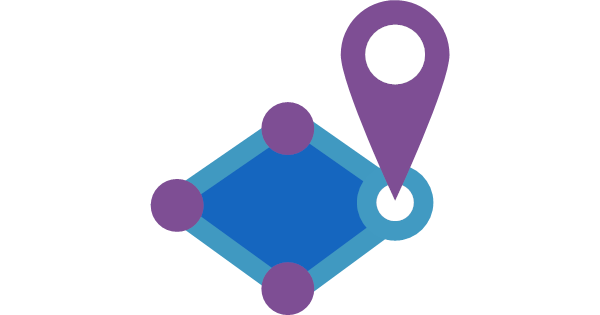
\includegraphics[height=2.5cm]{asa_logo.png}
    \caption{Logo di Azure Spatial Anchors}
\end{figure} \aCapo{}
Azure Spatial Anchors è un servizio di Microsoft mirato a fornire strumenti per sviluppare applicazioni in realtà aumentata su dispositivi iOS o Android predisposti per, rispettivamente, ARKit e ARCore, oppure su Microsoft HoloLens.\\
Permette di riconoscere spazi tridimensionali all'interno dei quali posizionare punti di interesse, chiamati Spatial Anchors, che possono essere salvati in cloud e poi recuperati, e possono essere messi in relazione a oggetti reali (come macchinari in un contesto industriale) o virtuali.

\subsection{ARCore}
\begin{figure}[ht]
    \centering
    
\includegraphics[height=2cm]{arcore_logo.png}
    \caption{Logo di ARCore}
\end{figure} \aCapo{}
ARCore, conosciuto anche come Google Play Services per AR, è un software development kit prodotto da Google per permettere lo sviluppo di applicazioni in realtà aumentata.\\
Si serve di tre componenti principali:
\begin{itemize}
    \item \textbf{6DOF:} il dispositivo sfrutta una piattaforma inerziale a sei assi per comprendere e tracciare la propria posizione relativa allo spazio;
    \item \textbf{Environmental understanding:} permette riconoscere dimensioni e locazione delle superfici lisce;
    \item \textbf{Light estimation:} permette al telefono di stimare le condizioni di luce dell'ambiente.
\end{itemize}
asa si appoggia proprio ad ARCore per implementare le proprie funzionalità di AR su Android.

\todo
\textcolor{todoOrange}{ar flutter plugin, sceneform?}


%**************************************************************
\section{Strumenti organizzativi}

\subsection{Slack}
\begin{figure}[ht]
    \centering
    
\includegraphics[height=1.5cm]{slack_logo}
    \caption{Logo di Slack}
\end{figure}
Slack è una piattaforma di comunicazione istantanea di proprietà di Salesforce e sviluppata da Slack Technologies per Windows, Linux, macOS, Android e iOS.\\
Permette di comunicare tramite messaggi, chiamate vocali e video, e di inviare media e files nelle chat private o nei canali. Quest'ultimi fungono da aggregatori e permettono di suddividere tematicamente la comunicazione.\\
\E{} inoltre possibile suddividere a un livello ancora più alto tramite i \textit{workspaces}, che aggregano al proprio interno utenti, canali e applicazioni: sono proprio quest'ultime che mostrano con maggiore chiarezza l'orientamento \textit{corporate} di Slack, infatti fornisce integrazione nativa con i maggiori software gestionali e organizzativi (come ad esempio Jira, Zoom, Drive, Outlook, etc).

\subsection{Github}
\begin{figure}[ht]
    \centering
    
\includegraphics[height=3cm]{github_logo}
    \caption{Logo di GitHub}
\end{figure}
GitHub è il più grande servizio di hosting di codice sorgente al mondo, abitualmente usato per sviluppare progetti open source, e fornisce vari servizi: version control di Git distribuito e access control, bug tracking, issue tracking, richieste di modifiche software, task management, integrazione continua e wiki per ogni progetto.\\ 
Permette inoltre, tramite forking, pull request e commenti, il miglioramento collaborativo del software, ad esempio risolvendo bug, aggiungendo funzionalità o migliorando quelle presenti.

